\documentclass{article}
\usepackage[utf8]{inputenc}
\usepackage[margin=1in]{geometry}
\usepackage{graphicx}
\usepackage{amsmath,amscd}
\usepackage{amssymb}
\usepackage{amsthm}
\usepackage{mathptmx}
\usepackage{color}

\author{Summarized by Sipu Ruan}
\title{Allowable Motion of Containment for Ellipsoid}

\begin{document}

\maketitle

\section{Mathematical Preliminary}
\subsection{General settings}
Let ${\bf a}=[a_1, a_2, ..., a_n]^T \in \mathbb{R}^n$ denotes the semi-axis of the smaller $n$ dimensional ellipsoid $E_a$, and so the semi-axis of bigger ellipse $E_b$ can be defined as ${\bf b}=[b_1,b_2, ..., b_n]^T=(1+\epsilon){\bf a}$, where $\epsilon \in (0,1]$ is the ``enlarging factor''. The $n$ dimensional ellipsoid can be implicitly represented by
\begin{equation}
({\bf x-t})^T A ({\bf x-t}) = 1 
\end{equation}
where ${\bf t} \in \mathbb{R}^n$ is the center position of the ellipsoid, and the eigenvalue decomposition of $A = R \Lambda^{-2} R^T$ gives a diagonal matrix $\Lambda$ whose diagonal entries are the lengths of semi-axis, and a rotation matrix $R \in SO(n)$ that represents the orientation of the ellipsoid. And the explicit expression can then be defined as
\begin{equation}
{\bf x} = R \Lambda {\bf u} + {\bf t}
\end{equation}
where ${\bf u}$ is the explicit expression of an $n$ dimensional unit sphere with the following properties
\begin{equation}
0 \leq {\bf u}_i^2 \leq 1; -1/2 \leq {\bf u}_i {\bf u}_j \leq 1/2 (i\neq j).
\end{equation}

\subsection{Pose Change Group and its Lie Algebra}
The rotation matrix and position vector introduced above forms a group called ``Pose Change Group'' (PCG) as $(R,{\bf t}) \in PCG(n)$. The corresponding Lie Algebra can be obtained by logarithm map as ${\bf \xi} = [{\bf \omega}^T, {\bf t}^T]^T \in \mathbb{R}^{n(n+1)/2}$, where ${\bf \omega}=\log^\vee(R)$ is the vector form of the matrix logarithm of the rotation matrix, which is a skew-symmetric matrix. The Lie Algebra can be transformed back to the Lie Group by exponential map, i.e. $(\exp(\hat{\bf \omega}), {\bf t}) \in PCG(n)$.

\subsection{Algebraic condition of containment}
By substituting the explicit expression of the moving smaller ellipsoid $E_a$ into the implicit expression of the larger ellipsoid $E_b$ that is fixed at the origin with orientation being identity, the algebraic condition for $E_a$ to move inside of $E_b$ without collision can be written as
\begin{equation}
\label{eq:condition_origin}
(R_a \Lambda({\bf a}) {\bf u} + {\bf t}_a)^T \Lambda^2({\bf b}) (R_a \Lambda({\bf a}) {\bf u} + {\bf t}_a) \leq 1.
\end{equation}

Once we enforce $\epsilon$ to be small, the rotation part calculated by exponential map can be approximated by the first order Taylor series as
\begin{equation}
\label{eq:rotation_approx}
R_a = \exp(\hat{\omega}_a) \approx \mathbb{I} + \hat{\omega}_a.
\end{equation}
Substituting Eq.~\ref{eq:rotation_approx} into Eq.~\ref{eq:condition_origin} and grouping parameters (${\bf u}$) and variables (${\bf \omega}$ and ${\bf t}$) gives the first-order approximation of the algebraic condition of containment as
\begin{equation}
\label{eq:condition_approx}
C({\bf \xi}) = {\bf \xi}^T H({\bf u}) {\bf \xi} + {\bf h}^T({\bf u}) {\bf \xi} + c({\bf u}) \leq 1, \text{  where ${\bf \xi} = [{\bf \omega}^T, {\bf t}^T]^T$.}
\end{equation}


\section{Closed-form Lower Bound of the Configuration Space}
This section reviews the closed-form solution of the allowable motion for the smaller ellipsoid. 

%%%%%%%%%%%%%%%%%%%%%%%%%%%%%%

\section{Configuration Space that has Larger Volume Generated via Convex Optimization}
To obtain a larger volume of the configuration space, we propose to construct the motion c-space further by a polyhedron shape. We first show that the expression of the algebraic condition is convex so that points lie inside the polyhedron defined by extreme points also satisfy the condition and further seek to find the extreme points to describe the shape of the c-space.

\subsection{Convexity of the first order approximation of the algebraic condition}
Since the first order approximation of the algebraic condition (\ref{eq:rotation_approx}) has to be satisfied for every ${\bf u}^{(i)}$ on the $n$ dimensional unit sphere, it is equivalent that the maximum value of $C({\bf \xi})$ has to satisfy the condition among all ${\bf u}^{(i)}$. So we seek to show that, instead, $\max C^{(i)}({\bf \xi})$ is convex as follows.

%%% Proof of claim %%%%
\begin{proof}	
For any fixed ${\bf u}^{(i)}$, we prove, at first, that the function $C^{(i)}({\bf \xi})$ is convex, which is to show that, given ${\bf \xi}_1, {\bf \xi}_2$
	
\begin{equation}
\label{proof_convex_ineq}
C^{(i)}(\alpha {\bf \xi}_1 + (1-\alpha) {\bf \xi}_2) \leq \alpha C^{(i)}({\bf \xi}_1) + (1-\alpha) C^{(i)}({\bf \xi}_2),  \forall  \alpha \in [0,1]
\end{equation}
	
Expanding both sides and moving right-hand side to the left gives
	
\begin{equation}
\label{proof_convex_each}
\begin{aligned}
& [LHS]-[RHS] \\
=& [(\alpha {\bf \xi}_1 + (1-\alpha) {\bf \xi}_2)^T H({\bf u}^{(i)}) (\alpha {\bf \xi}_1 + (1-\alpha) {\bf \xi}_2) + {\bf h}({\bf u}^{(i)})^T (\alpha {\bf \xi}_1 + (1-\alpha) {\bf \xi}_2) + c({\bf u}^{(i)})]\\
& - [\alpha ({\bf \xi}_1^T H({\bf u}^{(i)}) {\bf \xi}_1 + {\bf h}({\bf u}^{(i)})^T {\bf \xi}_1 + c({\bf u}^{(i)})) + (1-\alpha)({\bf \xi}_2^T H({\bf u}^{(i)}) {\bf \xi}_2 + {\bf h}({\bf u}^{(i)})^T {\bf \xi}_2 + c({\bf u}^{(i)}))] \\
=& -\alpha(1-\alpha) [({\bf \xi}_1 - {\bf \xi}_2)^T H({\bf u}^{(i)}) ({\bf \xi}_1 - {\bf \xi}_2)]
\end{aligned}
\end{equation}
	
The above expression satisfies the inequality $[LHS]-[RHS] \leq 0$ if and only if $({\bf \xi}_1 - {\bf \xi}_2)^T H({\bf u}^{(i)}) ({\bf \xi}_1 - {\bf \xi}_2) \geq 0$, or equivalently, $H({\bf u}^{(i)})$ is symmetric positive semi-definite, which can be showed by expanding the original expression of the condition to the 1st-order approximation as follows.
	
Since ${\bf \xi} = [{\bf \omega}^T, {\bf t}^T]^T$, only the quadratic terms with respect to both ${\bf \omega}$ and ${\bf t}$ from the 1st-order approximation will contribute to the calculation of ${\bf \xi}^T H({\bf u}^{(i)}) {\bf \xi}$ for any ${\bf \xi}$. Thus, we have, $\forall {\bf \xi} \in \mathbb{R}^{\frac{n(n+1)}{2}}$
	
\begin{equation}
\label{proof_convex_psd}
{\bf \xi}^T H({\bf u}^{(i)}) {\bf \xi} = (\hat{\omega}_a \Lambda({\bf a}) {\bf u}^{(i)} + {\bf t}_a)^T \Lambda^{-2}({\bf b}) (\hat{\omega}_a \Lambda({\bf a}) {\bf u}^{(i)} + {\bf t}_a)
\end{equation}
	
Since $\Lambda^{-2}({\bf b})$ is diagonal with non-negative entries on diagonal, \eqref{proof_convex_psd} $\geq 0$, which means that $H({\bf u}^{(i)})$ is symmetric positive semi-definite. Hence we showed the inequality condition for \eqref{proof_convex_each}, from which we conclude that each condition function $C^{(i)}({\bf \xi})$ is convex.
	
Next, we continue the proof by showing that the maximum of a family of convex functions is also convex. Since $C^{(i)}({\bf \xi})$ is convex, then taking maximum for both sides of \eqref{proof_convex_ineq} gives
	
\begin{equation}
\begin{aligned}
\max C^{(i)}(\alpha {\bf \xi}_1 + (1-\alpha) {\bf \xi}_2) &\leq \max [\alpha C^{(i)}({\bf \xi}_1) + (1-\alpha) C^{(i)}({\bf \xi}_2)],  \forall  \alpha \in [0,1]\\
&\leq \max \alpha C^{(i)}({\bf \xi}_1) + \max (1-\alpha) C^{(i)}({\bf \xi}_2),  \forall  \alpha \in [0,1] \\
\end{aligned}
\end{equation}
	
Thus $\max C^{(i)}({\bf \xi})$ is convex. 
\end{proof}
%%%%%%%%%%
And we can conclude that if for two extreme points ${\bf \xi}_1, {\bf \xi}_2$, $\max C^{(i)}({\bf \xi}_j) \leq 1, j=1,2$ are hold, then for points on the line segment between them, $\alpha {\bf \xi}_1 + (1-\alpha) {\bf \xi}_2, \forall \alpha \in [0,1]$, $\max C^{(i)}(\alpha {\bf \xi}_1 + (1-\alpha) {\bf \xi}_2) \leq \alpha \max C^{(i)}({\bf \xi}_1) + (1-\alpha) \max C^{(i)}({\bf \xi}_2) \leq 1$ is also satisfied. Hence points inside the convex hull of the extreme points also satisfy the algebraic condition, for which the small ellipsoid at each of those configurations does not collide with the larger one. 

\subsection{Finding extreme vertices that represent the polyhedron}
Now we search for the extreme points of the polyhedron by the following 2 cases: (1) extreme points that lies on each axis of the c-space; (2) points that are farthest to the origin.

Extreme points in each axis can be simply found by fixing the other axis lengths to zero. Since in each axis, there are 2 extreme points (positive and negative), we get $2N$ points for the first case, where $N$ is the dimension of the configuration space. 

For the vertices that are farthest to the origin, we seek to maximize the distance function to origin, i,e, $f = {\bf \xi}^T {\bf \xi}$. Further, the constraint is the algebraic condition (\ref{eq:condition_approx})
\begin{equation}
C({\bf \xi}) = {\bf \xi}^T H({\bf u}) {\bf \xi} + {\bf h}({\bf u})^T {\bf \xi} + c({\bf u}) \leq 1.
\end{equation}

Such constraint is a family of inequality constraints where ${\bf u}^{(i)}$ represents the $i$-th point on the boundary of a unit sphere. If we treat ${\bf \xi}$ as unknown variable and ${\bf u}$ as a group of known parameters, finding the maximum distance can be formed as an optimization problem as follows

\begin{equation}
\begin{aligned}
& {\bf \xi}_{extreme} = \arg\max {\bf \xi}^T {\bf \xi} \\
\text{{\bf s.t.   }} & C^{(i)}({\bf \xi}) = {\bf \xi}^T H({\bf u}^{(i)}) {\bf \xi} + {\bf h}({\bf u}^{(i)})^T {\bf \xi} + c({\bf u}^{(i)}) \leq 1 & (i=0,...,m)\\
\end{aligned}
\end{equation}
where, $m$ is the number of discretized points on the boundary of the unit sphere.

Since the objective function is quadratic, the solutions for each variable have 2 possibilities, so the total number of solutions can be up to $2^N$, where $N$ is the dimension of the configuration space. However, not all of those possibilities are feasible solutions, meaning we have to validate them by substituting back to the constraint inequalities.
%%%%%%%%%%%%%%%%%%%%%%%%%%%%%%

\section{Examples in 2D}
This section simulates the proposed closed-form lower bound and the extended solution for the configuration space in one rigid body 2D case.

\subsection{Closed-form c-space}
%%%%%%%%%%%%%%%%%%%%%%%%%%%%%%

\subsection{C-space generated via convex optimization}
\subsubsection{Mathematical settings}
At first, we find the extreme points at each c-space axis as follows. For the two translational axis ($x$ and $y$), the extreme points are located at $x_{extreme} = \pm \epsilon a_1$ and $y_{extreme} = \pm \epsilon a_2$ respectively. For the rotational axis ($\theta$), the extreme points can be found, in closed-form, as $\theta_{extreme} = \arctan (\pm \epsilon \sqrt[]{\frac{\alpha}{(\alpha(1+\epsilon)-1)(\alpha - \epsilon - 1)}})$ (please see Appendix ~\ref{apx:max_angle} for detailed derivations).

Then, for the farthest points to the origin, we apply the constraint convex optimization with $\xi = [\theta, x, y]^T$. Note that we might get 8 results since the cost function is quadratic, only 4 of them are valid by plugging back into the constraint functions. Thus, in total, we now get 10 extreme points to construct the polyhedron subspace from the configuration space.

\subsubsection{Numerical results}
Figs \ref{polyfit_cspace_10000samples} and \ref{polyfit_10000samples} show the numerical results of randomly sampled configurations of smaller ellipses that verify the above claim. The ellipse whose configuration point is inside the c-space polyhedron (convex hull of the 10 extreme vertices) lies safely inside the larger one without collision.

\begin{figure}[t]
\centering
\begin{minipage}[b]{0.4\textwidth}
	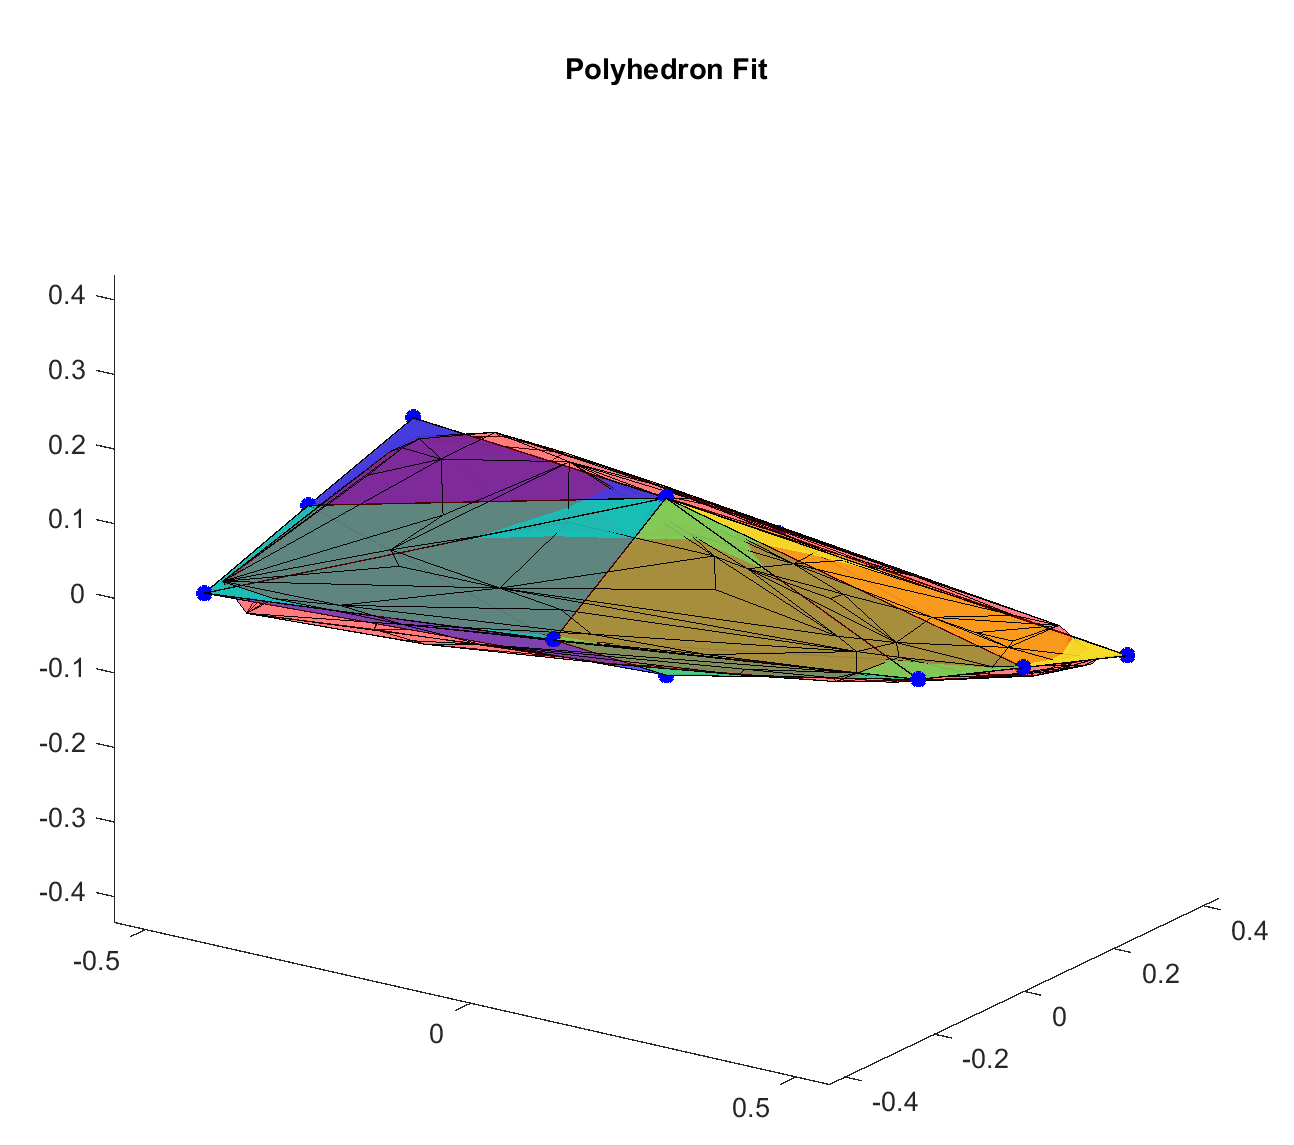
\includegraphics[scale = 0.2]{fig/c-space-polyhedron-fit.png}
	\caption{Heuristic fit as polyhedron represented by 10 extreme vertices, C-space}
	\label{polyfit_cspace}
	\end{minipage}
	\hfill
	\begin{minipage}[b]{0.4\textwidth}
		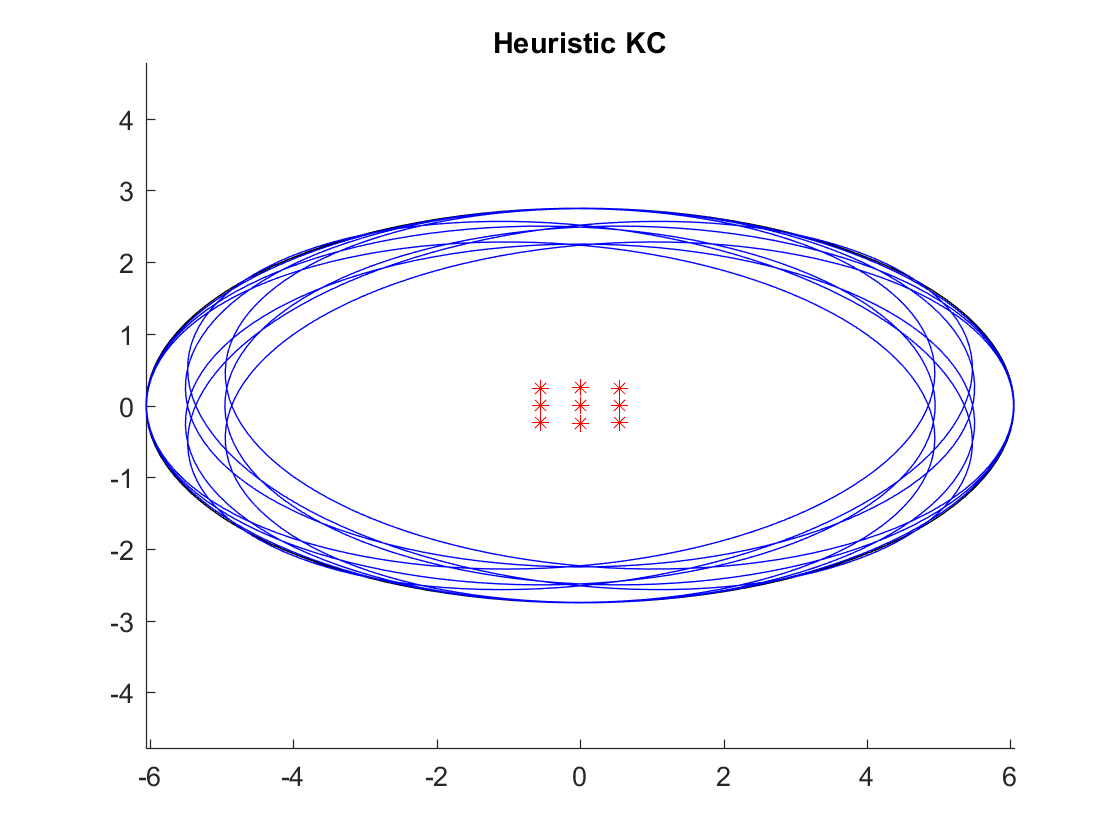
\includegraphics[scale = 0.25]{fig/ellipses-polyhedron-fit.png}
		\caption{Heuristic fit as polyhedron represented by 10 extreme vertices}
		\label{polyfit}
		\end{minipage}
\end{figure}

\begin{figure}[t]
	\centering
	\begin{minipage}[b]{0.4\textwidth}
		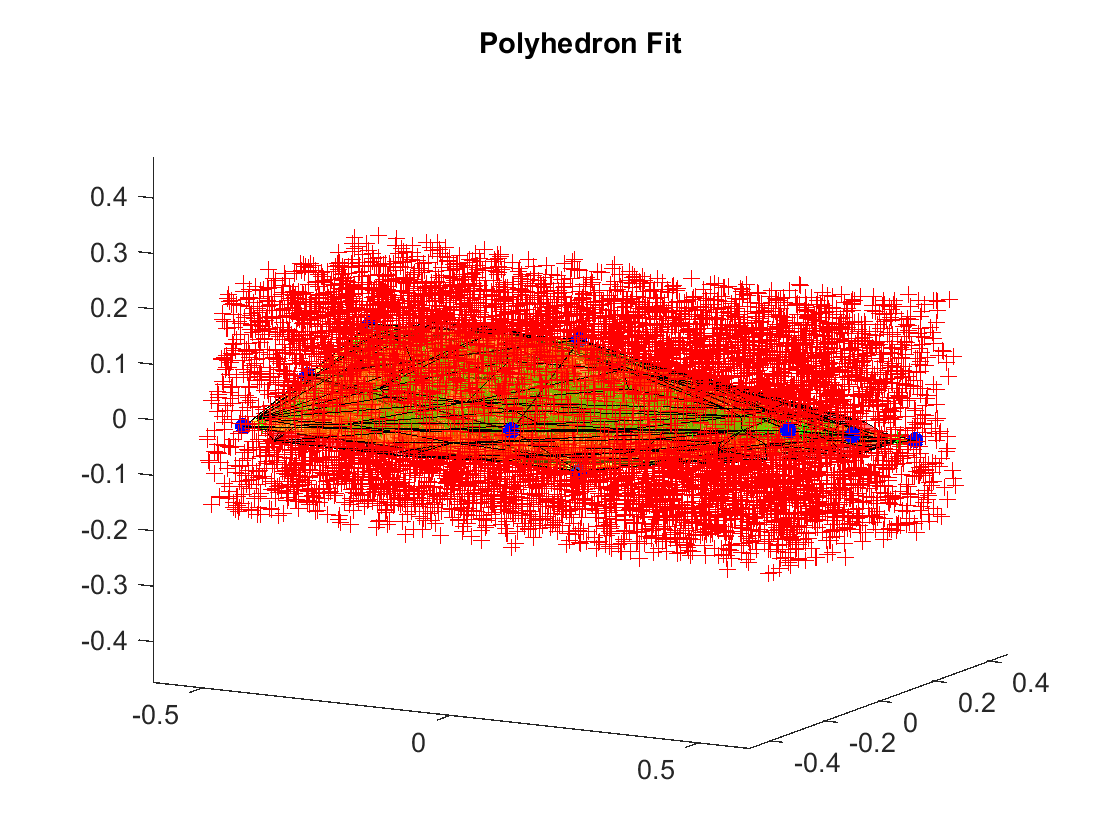
\includegraphics[scale = 0.2]{fig/c-space-polyhedron-fit-with-testPnts10000.png}
		\caption{C-space polyhedron fit with samples. Red: outside the convex hull; green: inside the convex hull}
		\label{polyfit_cspace_10000samples}
	\end{minipage}
	\hfill
	\begin{minipage}[b]{0.4\textwidth}
		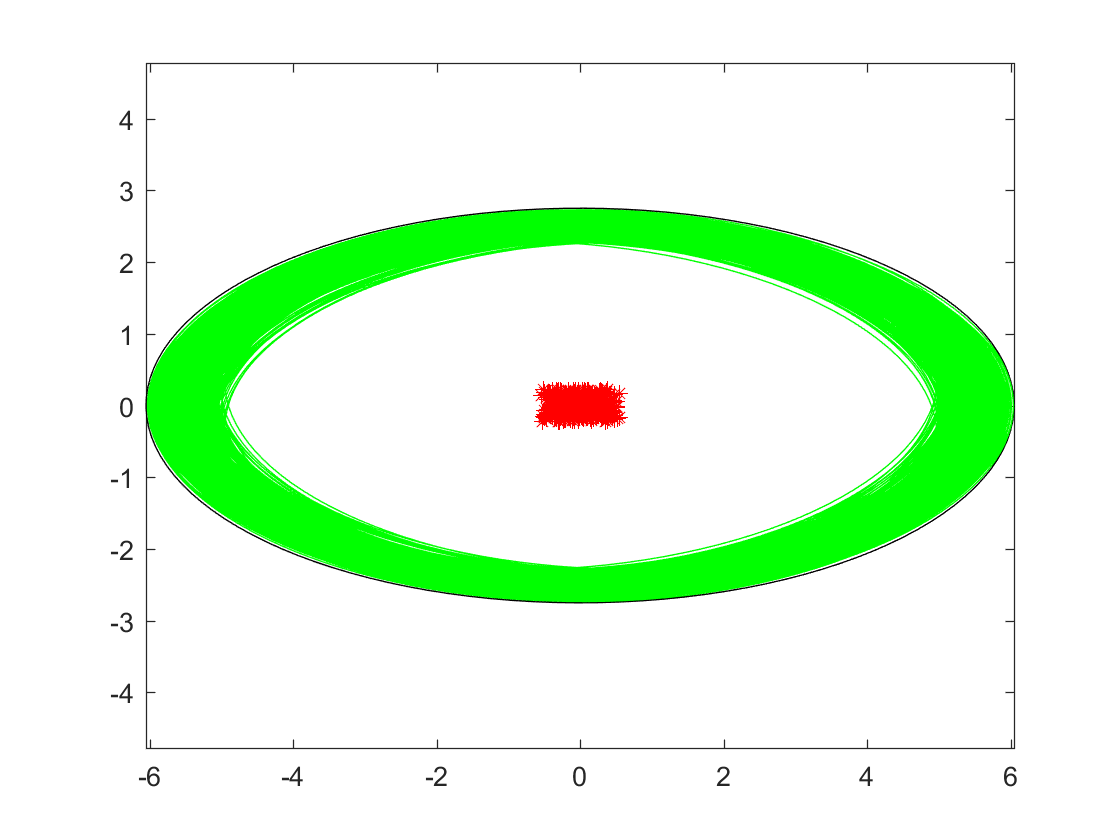
\includegraphics[scale = 0.25]{fig/ellipses-polyhedron-fit-with-testPnts10000.png}
		\caption{Smaller ellipses that lies safely inside the larger ellipse.}
		\label{polyfit_10000samples}
	\end{minipage}
\end{figure}
%%%%%%%%%%%%%%%%%%%%%%%%%%%%%%

\section{Examples in 3D}
In this section, we investigate the examples of the allowable motion c-space in 3D in closed-form and via convex optimization.

\subsection{Closed-form c-space}
\subsection{C-space generated via convex optimization}
\subsubsection{Mathematical settings}
The configuration space is now 6 dimensional, i.e $\xi = [\theta_1,\theta_2,\theta_3,x,y,z]^T$. The extreme points in translational axes are, similar to 2D, $x_{extreme} = \pm \epsilon a_1$, $y_{extreme} = \pm \epsilon a_2$ and $z_{extreme} = \pm \epsilon a_3$ respectively. To find the extreme points in rotational axes, we project the 3D space onto the three mutually perpendicular 2D planes, i.e. $x,y-$, $x,z-$, $y,z-$ plane. So the problem shrinks to the 2D case of finding the extreme rotational points at each plane, i.e. $\theta_i = \arctan(\pm \epsilon \sqrt{\frac{\alpha_i}{(\alpha_i(1+\epsilon)-1) (\alpha_i - \epsilon - 1)}}), i = 1,2,3$, where $\alpha_i$ is the aspect ratio of the projected ellipse at each plane. The number of extreme points is 12.

The extreme points with farthest distance to the origin can be obtained by the constraint convex optimization with the configuration variable defined above. In this case, we get 64 possible solutions and only 32 are valid. Combined with the extreme points at each axis, in total, we get 44 extreme points to create the 6D polyhedron.

\subsubsection{Numerical results}
Since it is not possible to visualize a 6D space, we divide the rotational and translational parts to split the whole space into two 3D spaces for visualization. Note that not all combinations of the extreme points in those two 3D spaces are valid, we still keep the 44 extreme configurations for the original 6D c-space. 



%%%%%%%%%%%%%%%%%%%%%%%%%%%%%%
%%%%%%%%%%%%%%%%%%%%%%%%%%%%%%
\appendix
\section{The maximum angle that the smaller ellipse can rotate}
\label{apx:max_angle}
The maximum angle that the smaller ellipse can rotate comes when the center point is fixed in the origin. And the angle can be found in closed-form as follows.

Assume the smaller and larger ellipse has semi-axis lengths ${\bf a}=[a_1,a_2]^T$ and ${\bf b}=[b_1,b_2]^T=(1+\epsilon){\bf a}$ respectively with the inflation factor $\epsilon$ and aspect ratio $\alpha=a_1/a_2$. We use the parametric forms for the two ellipses,
\begin{equation}
\begin{aligned}
{\bf u}_a = \left( 
\begin{aligned}
a_1 \cos \theta_a\\
a_2 \sin \theta_a
\end{aligned}
\right) &&
{\bf u}_b = \left( 
\begin{aligned}
b_1 \cos \theta_b\\
b_2 \sin \theta_b
\end{aligned}
\right)
\end{aligned}
\end{equation}

and the rotation of $E_a$ can be written as,
\begin{equation}
R(\phi) = \left(
\begin{aligned}
\cos\phi && -\sin\phi\\
\sin\phi && \cos\phi
\end{aligned}\right)
\end{equation}
where $\phi$ is the rotational angle of $E_a$.

Assume that the bigger ellipse $E_b$ is fixed with the world frame, with the center in the origin, and the larger semi-axis is aligned with x-axis. Then the points on the boundary of $E_b$ as seen in the world frame is exactly ${\bf u}_b$. Since $E_a$ only rotates around the origin, the points on its boundary as seen in the world frame should be $R(\phi) {\bf u}_a$.

The intersecting point of the two ellipses can be obtained by enforcing the two parametric equations as seen in the world frame to be equal as,
\begin{equation}
\begin{aligned}
& {\bf u}_b = R(\phi) {\bf u}_a \\
\iff & \left\{
\begin{aligned}
b_1 \cos\theta_b = a_1\cos\phi \cos\theta_a - a_2\sin\phi \sin\theta_a\\
b_2 \sin\theta_b = a_1\sin\phi \cos\theta_a + a_2\cos\phi \sin\theta_a
\end{aligned}
\right.\\
\end{aligned}
\end{equation}
Substituting $a_1 = \alpha a_2, b_1 = (1+\epsilon)a_1, b_2 = (1+\epsilon)a_2$, \textcolor{red}{and observing the fact that $\theta_b = \phi + \theta_a$ (rotational angle transformation from local frame to world frame of $E_a$) gives,}

%%%%%%%%%%%%%% WRONG!! %%%%%%%%%%%%%%%% 
\begin{equation}
\begin{aligned}
& \left\{
\begin{aligned}
\alpha a_2 (1+\epsilon) \cos(\theta_a + \phi) = \alpha a_2 \cos\phi \cos\theta_a - a_2\sin\phi \sin\theta_a\\
a_2 (1+\epsilon) \sin(\theta_a + \phi) = \alpha a_2 \sin\phi \cos\theta_a + a_2\cos\phi \sin\theta_a
\end{aligned}
\right. \\
\iff & 
\left\{
\begin{aligned}
\alpha \epsilon \cos\theta_a \cos\phi = (\alpha(1+\epsilon) - 1) \sin\theta_a \sin\phi \\
\epsilon \sin\theta_a \cos\phi = (\alpha - \epsilon - 1) \cos\theta_a \sin\phi \\
\end{aligned}
\right. \\
\end{aligned}
\end{equation}
Since always $a_2 < b_2$, the points on smaller semi-axis of the smaller ellipse will be always inside the bigger ellipse, so when we consider the case of intersecting, $\theta_a \neq \pi/2$, or $3\pi/2$, or $\cos\theta_a \neq 0$. Further, One sufficient condition when two ellipses intersect should be $a_1 \geq b_2$, or $\alpha \geq 1+\epsilon$, and the equal sign occurs only when $\phi = \pi/2, 3\pi/2$ and $\theta_a = 0, \pi$, or $\cos\phi = 0$ and $\sin\theta_a = 0$.

So, for general cases, we could rearrange the above system of equations as,
\begin{equation}
\left\{
\begin{aligned}
\frac{\alpha \epsilon}{(\alpha(1+\epsilon)-1)} = \tan\theta_a \tan\phi \\
\frac{\epsilon}{(\alpha - \epsilon - 1)} \tan\theta_a = \tan\phi
\end{aligned}
\right.
\end{equation}
Since $b_1 \geq a_1$, $\phi \neq 0, \pi$ ($\tan\phi \neq 0$) when two ellipses intersect, then we could get,
\begin{equation}
\begin{aligned}
& \frac{\alpha \epsilon}{(\alpha(1+\epsilon)-1) \tan\phi} = \frac{(\alpha - \epsilon - 1) \tan\phi}{\epsilon}\\
\Rightarrow & \tan^2\phi = \frac{\alpha \epsilon^2}{(\alpha(1+\epsilon)-1)(\alpha - \epsilon - 1)}
\end{aligned}
\end{equation}
Solving for $\phi$ gives,
\begin{equation}
\phi = \arctan (\pm \epsilon \sqrt[]{\frac{\alpha}{(\alpha(1+\epsilon)-1)(\alpha - \epsilon - 1)}})
\end{equation}

Figures \ref{diff-alpha} and \ref{diff-epi} show the numerical experiments to verify the result, with different $\alpha$ and $\epsilon$ values respectively.

\begin{figure}
\centering
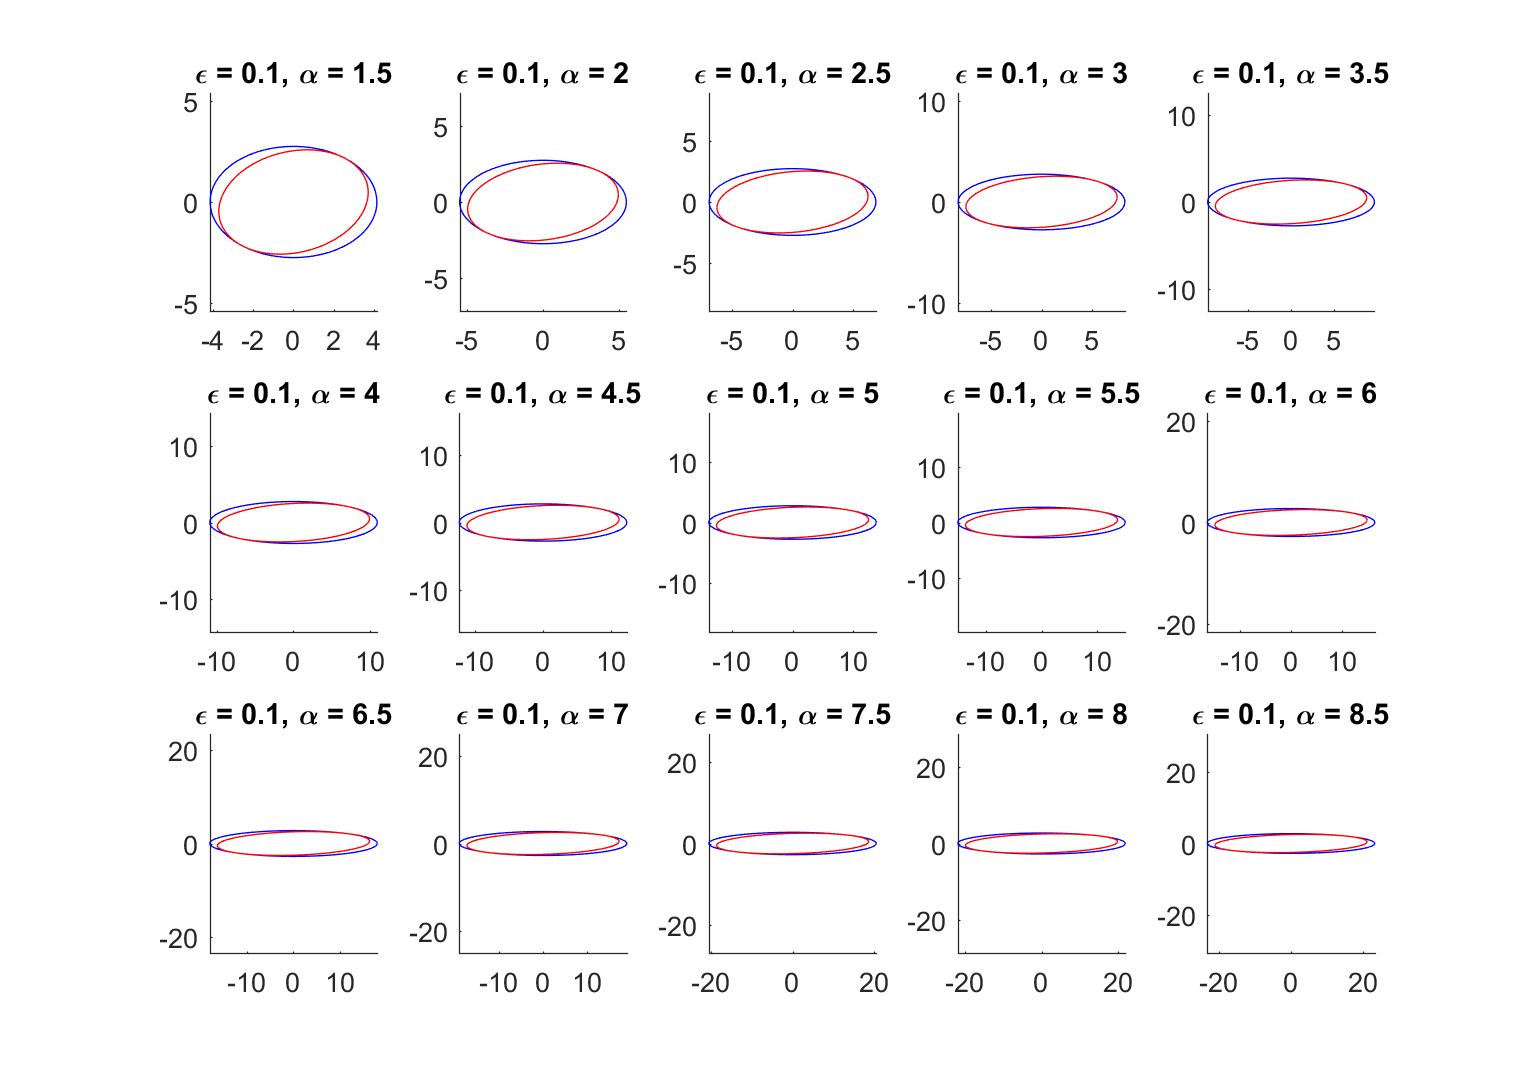
\includegraphics[scale = 0.4]{fig/closed-form_maxAngle-test_alpha.png}
\caption{Test with different values of aspect ratio $\alpha$, fixed $\epsilon = 0.1$}
\label{diff-alpha}
\end{figure}
	
\begin{figure}
\centering
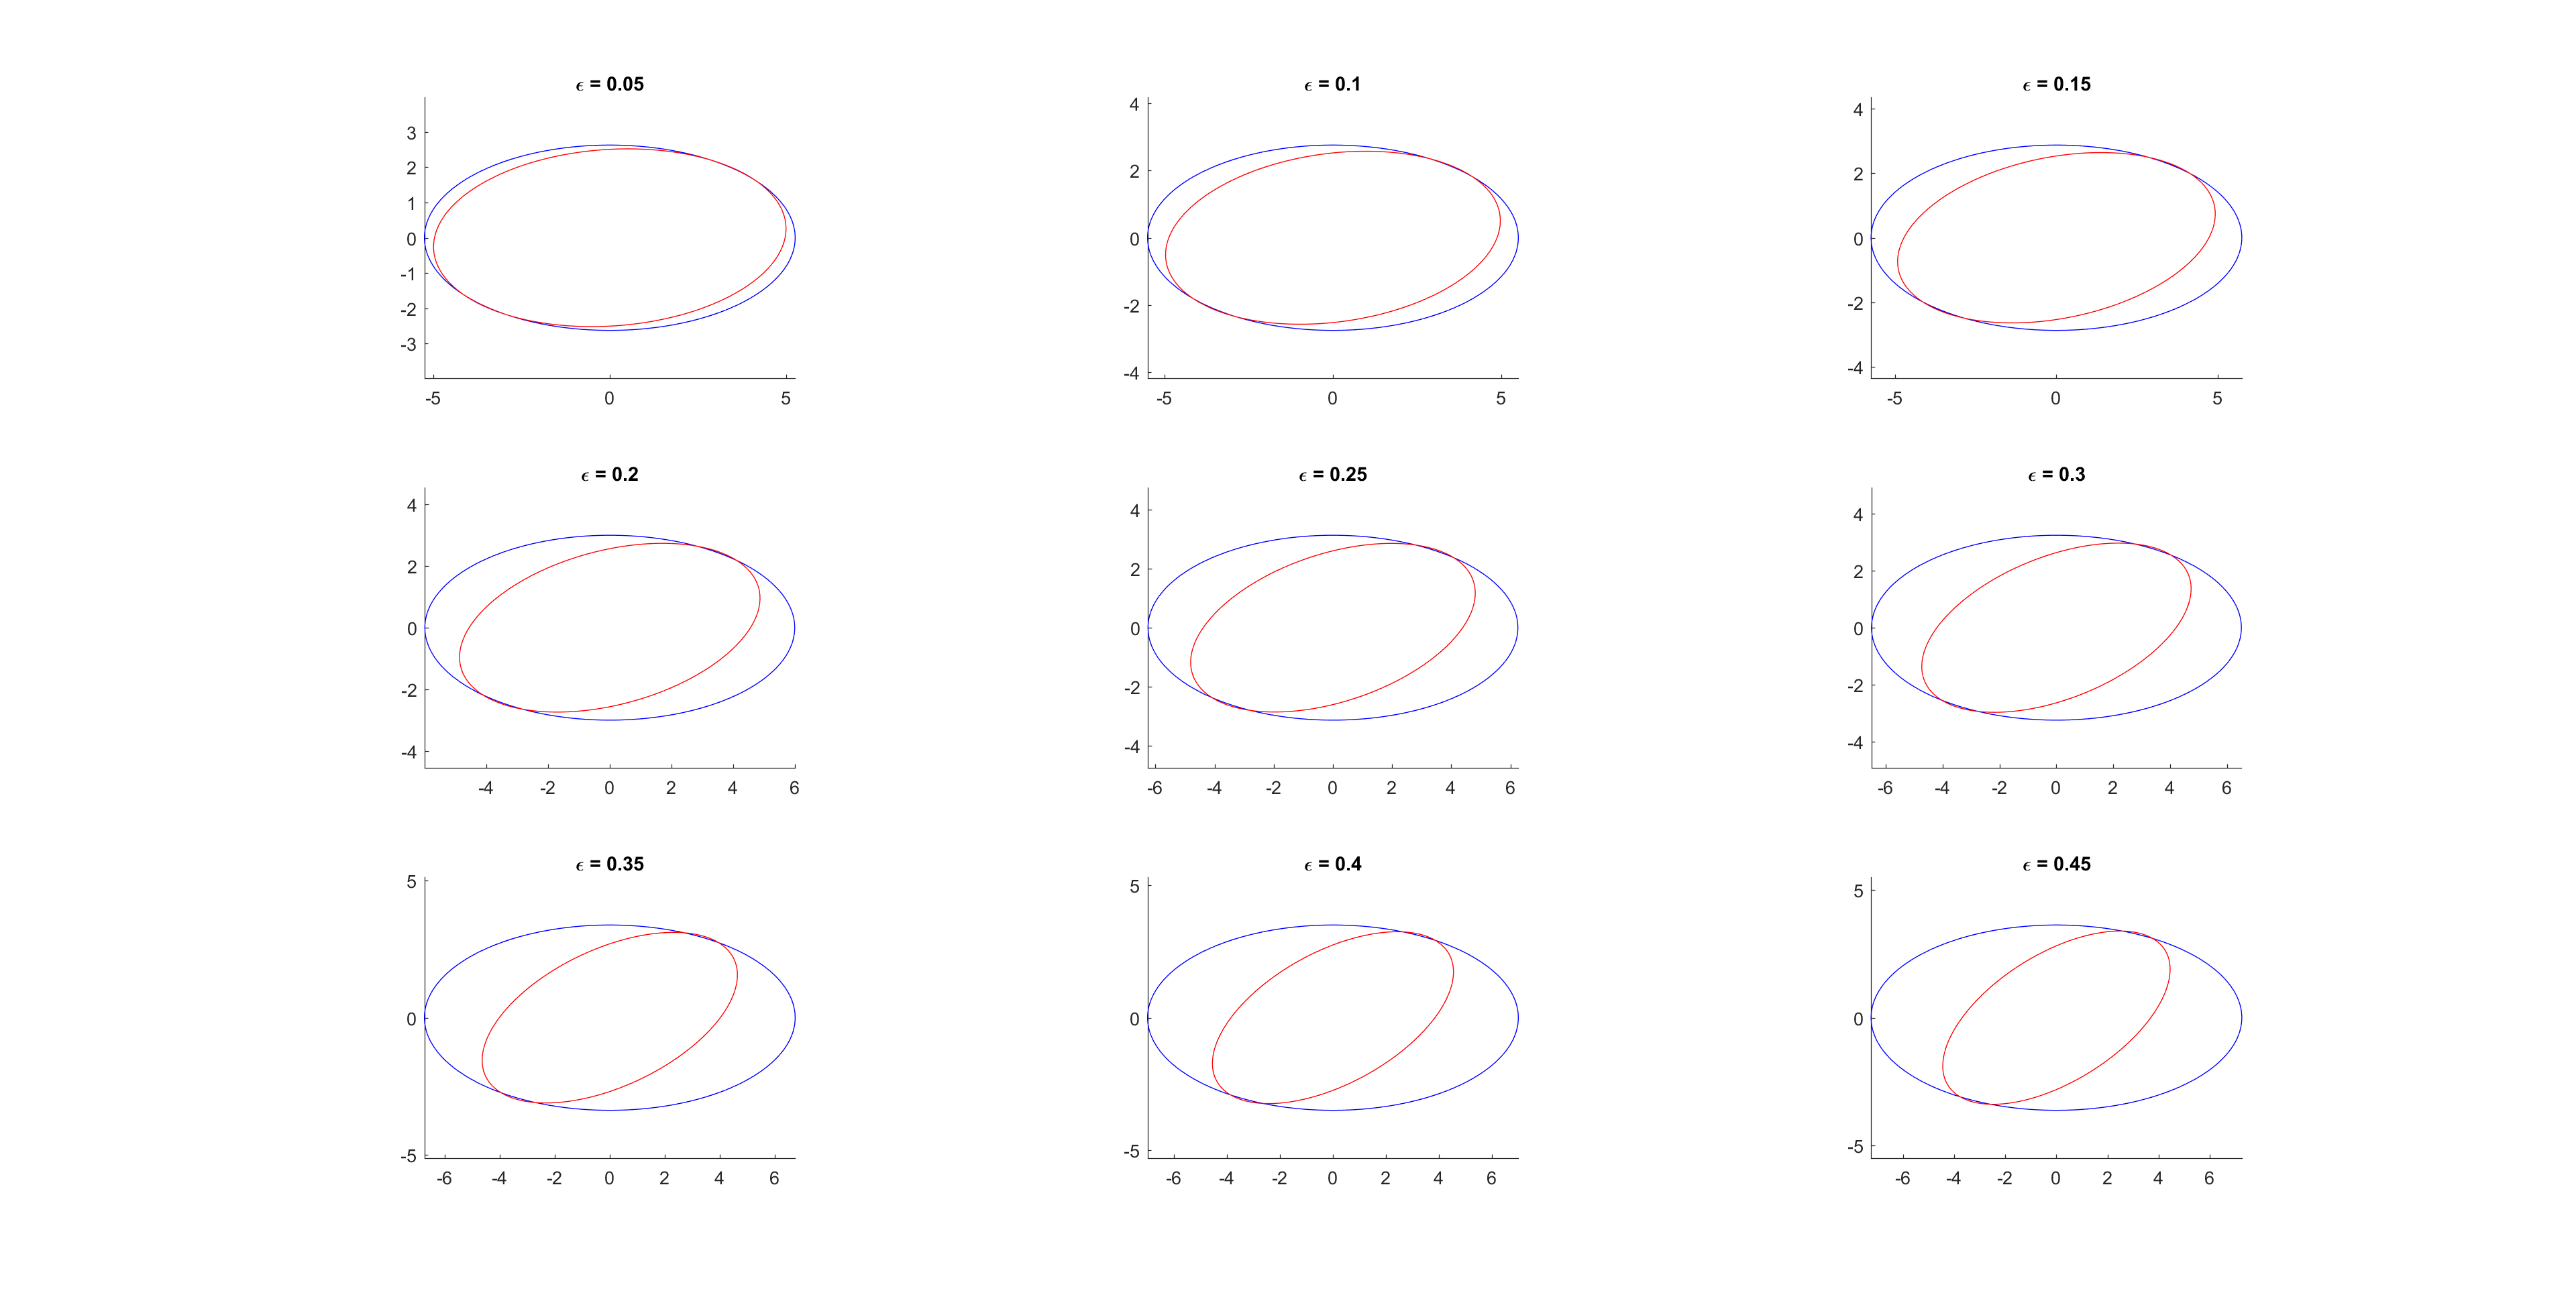
\includegraphics[scale = 0.4]{fig/closed-form_maxAngle-test_epsilon.png}
\caption{Test with different values of explode factor $\epsilon$, fixed $\alpha = 2$}
\label{diff-epi}
\end{figure}
%%%%%%%%%%%%%%%%%%%%%%%%%%%%%%
\end{document}
